\chapter{Galaxy SED fitting methods and applications}\label{chp:sed}

\begin{flushright}
  {\em ``Everything we see hides another thing, we always want to see\\ what is hidden by what we see.''}\\

\ \

\normalsize
{Ren\'e Magritte}  
\end{flushright}


\noindent{\emph{The work presented in this Chapter contains part of {\bf Palmese et al., 2018}, currently in the DES review process, and of my contribution to the SV public release and DES SV papers with photometric redshift estimation with ANNz2. The machine learning method for stellar mass estimation is unpublished.}}

%\section{Introduction}
Fundamental properties of the unresolved stellar populations within galaxies are encoded in the galaxy Spectral Energy Distribution (SED) that we observe. These include the Star Formation History (SFH), stellar mass, initial mass function (IMF) and the metallicity. These information are further folded in with the redshift of galaxies. Extracting as much information as possible from the DES galaxy SEDs is the first goal of this thesis, as the derived properties are fundamental to the analyses that we want to make for gravitational wave source host galaxies and clusters. Thankfully, a huge effort has been spent by the astrophysical community to model and fit SEDs of unresolved stellar populations over the past decades.
In this Chapter we first provide an introduction to redshift estimation and stellar population synthesis models, then we describe the methods used in this thesis to evaluate galaxy properties, from photometric redshifts to stellar masses and star formation rates. In particular, we present a code written by James Annis and myself that uses Bayesian Model Averaging to evaluate galaxy properties that we have made publicly available. We show the first application of machine learning methods to stellar mass estimates from photometric data. Finally, we present some applications of these methods with DES data.

\section{Redshifts}
We recall that the redshift of a galaxy is defined in Eq. (\ref{eq:z}) as:
\begin{equation}
z\equiv \frac{\lambda_{\rm oss}}{\lambda_{\rm em}}-1\,
\end{equation}
but not all of it is due to the expansion of the Universe as in Eq. (\ref{eq:z}). The redshift of a galaxy includes contributions coming from the cosmological redshift due to the expansion of the Universe ($z_H$), from peculiar motions with respect to the observer ($z_{\rm phys}$) and possibly to gravitational redshifts ($z_{\rm grav}$, due to galaxies motion within gravitational potential wells), so that:
\begin{equation}
z_{\rm tot} = z_H+z_{\rm phys}+z_{\rm grav}\,.
\end{equation}
The gravitational redshift is usually neglected as it is a very small contribution to the total redshift.\footnote{Works on gravitational redshifts in clusters and galaxies have tried to estimate this contribution through statistical methods such as stacking (e.g. \citealt{wojtak}; \citealt{sadeh15}).}. Peculiar motions can arise from the motion of Earth around the Sun (with a velocity of $\sim 29~{\rm km~s^{-1}}$), the Milky Way's motion with respect to the CMB reference frame ($\sim 630 ~{\rm km~s^{-1}}$ corresponding to $z \sim 0.002$) and orbital motions of galaxies around each other or in cluster potential wells. The galaxies' velocity dispersion in clusters can reach values of $\sim 1500 ~{\rm km~s^{-1}}$ (corresponding to $z\sim 0.005$).

Photometric surveys such as DES measure the redshift of galaxies through photometry, and the estimated redshifts are called photometric redshifts or photo-$z$'s. Photo-$z$'s have been introduced back in the 60's by \citet{baum}, and they have been extensively studied and utilised since the advent of the recent wide-field photometric surveys. While spectroscopy can produce more precise redshift measurements, it is technically an arduous work to measure spectra for hundreds of millions of galaxies in a reasonable time span with current technology. While a whole region of galaxies can be imaged with DECam at once, spectroscopy can only be obtained for those galaxies that can be targeted with slits or fibers. Even though photo-$z$'s are subject to large uncertainties, some analyses, such as weak lensing, can benefit more from larger number statistics than from precise redshift measurements. The requirements on the photo-$z$ accuracy for a galaxy survey are usually computed from the requirements on the estimates of cosmological parameters. The requirements on DES redshifts are defined through several metrics computed for a sample of galaxies that has both a photo-$z$ estimate and a reference redshift given by spectroscopy. We assume that those spectroscopic redshifts are the true redshifts of galaxies. The metrics are defined in \citet{sanchez}:
\begin{itemize}
\item $\overline{\Delta z}$: the mean of the bias distribution $\Delta z$, given by the difference between estimated photo-$z$'s and the reference redshifts.
\item $\sigma_{\Delta z}$: the standard deviation of the bias distribution.
\item $\sigma_{68}$: the scatter expressed as the half--width of the bias distribution around the median of the $\Delta z$ distribution, containing $68\%$ of the galaxies. This scatter is supposed to be $<0.12$ for DES.
\item ${\rm out}_{2\sigma}$: the outlier fraction, i.e. the fraction of galaxies with $|\Delta z - \overline{\Delta z}|>2\sigma_{\Delta z}$, which is required to be $<0.1$.
\item ${\rm out}_{3\sigma}$: the fraction of galaxies with $|\Delta z - \overline{\Delta z}|>3\sigma_{\Delta z}$, which is required to be $<0.015$.
\end{itemize}

\begin{figure}\centering
\includegraphics[width=0.5\textwidth]{/Users/palmese/work/PhD_thesis/thesis_format/chapters/chapter2/figs/filters.jpg}\caption{DECam $griz$ filters with a galaxy spectrum redshifted from $z=0$ to $z=1$. The 4000 \AA~ break can be measured with DECam filters over this redshift range. From the DES Figures library.}\label{fig:filtersz}
\end{figure}

One of the main features of galaxies' SEDs that allow us to measure redshifts with DES is the relatively sharp drop at 4000 \AA: the 4000 \AA~ break. This feature is produced by the absorption of various metallic lines around similar wavelengths, and can be further enhanced by a deficiency of young, blue stars (e.g. \citealt{1985ApJ...297..371H}). The drop is shown in the blue line in Figure \ref{filters}, which represents the spectrum of a typical galaxy at $z=0$. For more distant galaxies the 4000 \AA~ break is shifted towards longer wavelengths, as shown in green and red lines in the plot. This feature is covered by the DES filters out to $z\sim 1$, and this is why we usually do not go beyond this redshift with DES analyses.

For what concerns DES galaxy evolution and clusters studies, objects are usually at cosmological distances (mostly $0.1<z<1$) so that the only contribution to the redshift that we consider from photometric data is due to the Hubble expansion. The remaining parts are negligible compared to $z_H$ and well below our photometric redshift uncertainty. GW follow up studies are an exception, as GW sources are in the local universe (usually $z<0.1$) and the redshift estimation becomes tricky with DES data alone, so that we require spectroscopic data. The Supernova rejection study is exempted from a spectroscopic follow up as it falls again into the cosmological distance regime.

It is worth noting that in some analysis, estimation of the full redshift probability density function (PDF) may be useful (or even just a random draw from it). Some redshift estimation codes are able to provide that as their output, although storing and sharing a full PDF for each entry in a large galaxy sample such as DES is an known issue (see e.g. \citealt{rau}).

\section{Stellar population synthesis modeling}\label{sec:SPS}
The spectral evolution of galaxies is usually studied through what we call ``Stellar Population Synthesis'' (SPS) modeling, or ``evolutionary synthesis'' modeling. These method relies on stellar evolution models to constrain stellar populations with a certain metallicity and age; the first synthesis models of this type were developed in the late 60's and 70's (e.g. \citealt{tinsley}; \citealt{tinsley72}; \citealt{searle}).  Note that in the following we describe a commonly used methodology, but it is not universal. 

\begin{figure}\centering
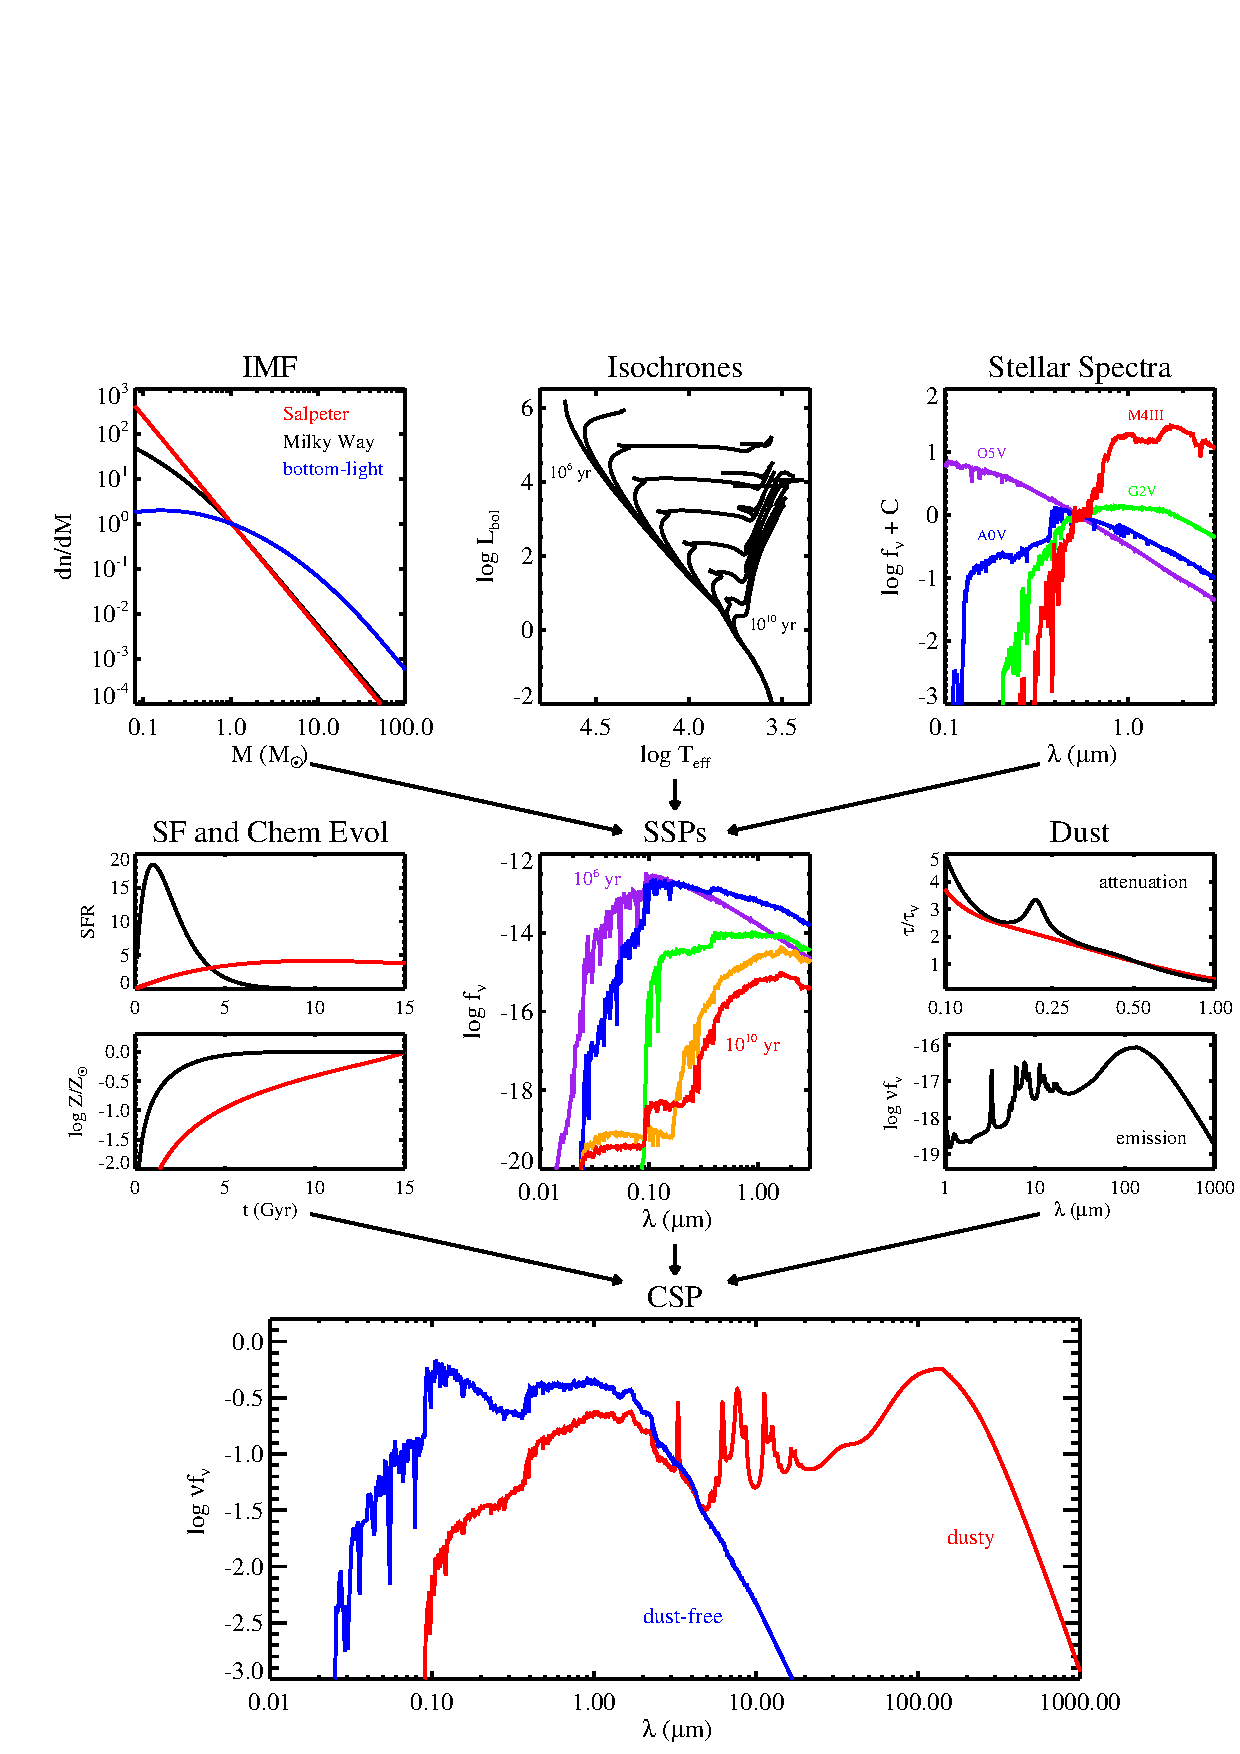
\includegraphics[width=0.7\textwidth]{/Users/palmese/work/PhD_thesis/thesis_format/chapters/chapter2/figs/f1.pdf}\caption{Schematic illustration of stellar population synthesis modeling, from \citet{conroy}.}\label{fig:csp}
\end{figure}

\subsection{Simple stellar populations}
The first step in constructing SPS models is building the simple stellar population (SSP) models, i.e. the evolution over time of a stellar population having a single metallicity and age. The time $t$ and metallicity\footnote{The mass fraction in elements heavier than helium.} $Z$ dependent SED of an SSP $f_{\rm SSP}$ writes as (\citealt{conroy}):

\begin{equation}
f_{\rm SSP} (t,Z) = \int^{m_{\rm up}}_{m_{\rm lo}} f_{\rm star}[T_{\rm eff} (M_\star), {\rm Log} ~g(M_\star)|t,Z] \phi(M_\star) {\rm d} M_\star\, , \label{eq:ssp}
\end{equation}
where $M_\star$ is the stellar mass at the zero--age main sequence.
The ingredients that go into Eq. (\ref{eq:ssp}) are:
\begin{itemize}
\item Isochrones from a stellar evolution theory. Isochrones represent the position of stars in the Hertzsprung--Russell diagram with same age and metallicity. The theory has some lower and upper limits ($m_{\rm lo}$ and $m_{\rm up}$ ) on stellar masses and the isochrones dictate the relation between the effective temperature $T_{\rm eff}$, the surface gravity $g$ and $M_\star$ at each time and metallicity values. Some popular isochrones include the Padova (\citealt{bertelli}; \citealt{girardi}) and the BaSTI (\citealt{pietrinferni}) models.
\item Stellar spectra $f_{\rm star}$. These are derived from stellar spectral libraries, that deal with converting the stellar evolution outputs into actual spectral energy distributions. Usually several libraries are used together in order to cover a wider range of the parameter space. Libraries can be theoretical (e.g. BaSeL, \citealt{basel1}, \citealt{basel2}, \citealt{basel3} which is the most used theoretical stellar library) or empirical (e.g. STELIB, \citealt{stelib}, MILES, \citealt{miles}).
\item The Initial Mass Function $\phi(M_\star)$, which gives the stellar mass distribution of the zero--age main sequence. Typically, this has the form of a power law or a broken power law. A set of widely used IMFs is discussed in Chapter 6.
\end{itemize}
The choice of the IMF is an important step as the IMF not only determines the normalization of the $M_\star/L$, but it also significantly impacts composite stellar populations SEDs. In fact, the luminosity of an SSP is dominated by the stars at the turnoff mass, which translates into a range of several turnoff masses within a composite population. The most widely used IMFs differ at the low mass end ($M_\star <1 M_\odot$): stars in this regime dominate the stellar mass of a galaxy but contribute very little (a few percent) to the overall galaxy bolometric luminosity for an old stellar population. It is thus impracticable to discern between these different models with the photometric data from DES without introducing degeneracies with stellar mass/mass-to-light ratio.

\subsection{Composite stellar populations}

A galaxy's spectrum can be built up by adding the spectra of several SSPs of different ages and metallicities into a Composite Stellar Population (CSP) model of the form:

\begin{equation}
f_{\rm CSP} (t) = \int^{t'=t}_{t'=0} \int^{Z_{\rm max}}_{Z=0} \big(  f_{\rm SSP}(t',Z)  SFR(t-t')P(Z,t-t')e^{-\tau_d(t')}+Af_{\rm dust}(t',Z) \big){\rm d} t' {\rm d} Z\, ,\label{eq:csp}
\end{equation}
The ingredients needed to build such SED are:
\begin{itemize}
\item The star formation history (SFH), that dictates the ages of stars from SSPs. This is given in the form of a star formation rate (SFR) as a function of time. Widely adopted SFHs include very simplystic models, such the exponential or $\tau$ model (\citealt{schmidt}), that follows SFR$(t)\propto {\rm e}^{-t/\tau}$. A more realistic SFH includes an early rising SFR as SFR$(t)\propto t^\beta {\rm e}^{-t/\tau}$. In this thesis we adopt more complicated models that include log-normal and \citet{simha} models.
\item A time--dependent metallicity distribution $P(Z,t)$, which is often reduced to a $\delta$--function, i.e. a single metallicity value.
\item A dust model. Interstellar dust has an important effect on galaxies' SEDs through UV--to--NIR obscuration and IR emission, and the impact is stronger for star--forming galaxies. Usually, when modeling SPS we fix the shape of the attenuation curve to a \citet{calzetti} or a \citet{charlotfall} law and fit for the normalization. The dust attenuation enters in Eq. (\ref{eq:csp}) through the dust optical depth $\tau_d$. Dust emission is modeled through $f_{\rm dust}$, including a normalisation constant $A$.
\end{itemize}
We call stellar mass of a galaxy the total amount of mass in stars it contains. This quantity is usually measured from a mass-to-light ratio $M_\star/L$ derived from some SED fitting and then multiplied by the luminosity.
Figure \ref{fig:csp} shows all the components necessary for building a CSP model. For a comprehensive review on SPS models see \citet{conroy}.

Synthetic photometry can then be derived from the computed spectra $F(\lambda)$ by integrating them after convolution with the filters transmission curves $S(\lambda)$. The derived fluxes or magnitudes can then be compared with the observed values to constrain galaxy properties. For a filter $i$ with transmission curve $S_i(\lambda)$, the magnitude is given by (e.g. \citealt{girardi}):

\begin{equation}
m =  -2.5~{\rm Log}\Big( \frac{\int\frac{\lambda}{hc}F_\lambda S_i(\lambda){\rm d} \lambda}{\int\frac{\lambda}{hc}F^0_\lambda S_i(\lambda){\rm d} \lambda} \Big)\, ;\label{eq:mag}
\end{equation}
where the factors $\frac{\lambda}{hc}$ come from the fact that photons are counted in CCD cameras, and $F^0_\lambda$ is a normalisation that depends on the magnitude system used. In this thesis and more in general in DES, we usually work with magnitudes in the AB system, which is normalised so that a spectrum with constant flux per unit frequency has zero magnitude. This translates into $F^0_{AB}(\nu)=3.631\times 10^{-20} {\rm erg~s^{-1}~cm^{-2}~Hz^{-1}}$ and $F^0_{AB}(\lambda)=F^0_{AB}(\nu)c/\lambda^2$.

\section{Methods}\label{sec:zmethods}
There are two common approaches to photo-$z$'s  estimation: template--fitting methods and machine learning methods. 

{\bf Template fitting} methods involve the compilation of a library of expected magnitudes for a range of galaxy spectra over a grid of redshifts. The latter can be either synthetic (e.g. \citealt{bc03}; \citealt{fsps}), as described in Section \ref{sec:SPS}, or empirical (e.g. \citealt{cww}). The expected magnitudes $t_i$ for each $i$-th filter are estimated through Eq. (\ref{eq:mag}) and compared to the observed ones, $m_i$, with error $\sigma_i$. The fit can be performed through a $\chi^2$ minimization, so minimizing:
\begin{equation}
\chi^2(z,{\rm SED})=\sum_i \Bigg( \frac{m_i-\alpha(z,{\rm SED}) t_i(z,{\rm SED}) }{\sigma_i} \Bigg)^2 \,,
\end{equation}
with respect to redshift and template SED allows to find the best--fit SED at redshift $z$. The scaling factor $\alpha(z,{\rm SED})$ normalises the template magnitudes to the observed ones:
\begin{equation}
\alpha (z,{\rm SED})=\Bigg( \sum_i \frac{m_i~t_i(z,{\rm SED}) }{\sigma_i^2} \Bigg)/ \Bigg( \sum_i  \frac{t_i(z,{\rm SED}) }{\sigma_i^2} \Bigg) \,.
\end{equation}
Examples of template--fitting methods are \textsc{HyperZ} (\citealt{hyperz}), \textsc{EAZY} (\citealt{eazy}), \textsc{LePhare} (\citealt{ilbertlephare}) and BPZ (which also incorporates priors through a Bayesian method; \citealt{bpz}).

{\bf Machine learning} (ML) techniques attempt to determine a mapping from colour space to redshift through training on spectroscopic data. The mapping can be reproduced with a simple polynomial fit (\citealt{connolly}) or though more complicated relations, such as those arising from artificial neural networks (ANNs). Examples of codes using neural networks are \textsc{ANNz} (\citealt{annz}), \textsc{ANNz2} (\citealt{annz2}) and \textsc{skynet} (\citealt{skynet}), while \textsc{tpz} (\citealt{tpz}) uses random forests.

One of the main concerns with machine learning derivation of redshifts for deep photometric surveys such as DES is the incompleteness of the training sample. This relates to the incompleteness of the spectroscopic data, in other words to the unrepresentativeness of the galaxies from photometric data. In particular this is a real problem towards the faint end of galaxy samples, where there is a lack of spectroscopy. Several studies have tried to mitigate this problem, for example through means of galaxy colours weighting (\citealt{lima}). On the other hand, also with template--fitting methods one needs to be careful that the library used is representative for the observed data, and that synthetic SEDs are realistic.

As far as we are concerned, machine learning methods have been extensively used to estimate redshifts from photometric data, but not other parameters  that go into the galaxy evolutionary modeling described in the previous Section. Principal Components Analysis (PCA) and machine learning techniques have been applied to spectroscopic data (e.g. \citealt{wisconsin}), in particular to solve classification problems (e.g. \citealt{quenching}), and for morphological studies (\citealt{gauci}; \citealt{schutter}). We decided to apply for the first time a machine learning method to estimate stellar mass from photometric surveys. The same method could ideally be applied to any other quantity that can enters the evolutionary synthesis models.

In this Section we therefore describe the methods used in this thesis as SED fitting methods, rather than simply photo-$z$ estimation codes, as we use them to derive galaxy properties beyond the photo-$z$'s. 

\subsection{Bayesian Model Averaging algorithm}\label{sec:BMA}

A major cause of uncertainty in stellar mass estimation from broadband photometry is in the model assumptions (see e.g. \citealt{mitchell}) that are needed in model fitting techniques. These assumptions mainly involve redshift, star formation history (SFH), the initial mass function, the dust content and the knowledge of stellar evolution at all stages. 
We therefore choose not to ignore the uncertainty on model selection and use a set of robust, up-to-date stellar population synthesis (SPS) models and average over all of them, marginalizing over the model uncertainty. The method used here is called Bayesian Model Averaging (BMA, see e.g. \citealt{hoeting}). BMA has already been successfully applied to galaxy SED fitting  parameter estimation in \citet{taylor}.

Our code can be used to estimate physical parameters of galaxies (stellar masses, specific star formation rates, ages, metallicities) as well as cluster stellar masses and total SFR (when provided with cluster membership probabilities), and it is publicly available at \url{https://github.com/palmese/BMAStellarMasses}.

%\subsubsection{Bayesian Model Averaging}
The BMA  starting point is Bayes' theorem, through which we can write the posterior probability distribution $p(\bar{\theta}_k|D,M)$ of the set of parameters $\bar{\theta}_k$ given the data $D$ and the model $M_k$:
\begin{equation}
p(\bar{\theta}_k|D,M_k)=\frac{p(D|M_k,\bar{\theta}_k)p(\bar{\theta}_k|M_k)}{p(D|M_k)}\,,
\end{equation}
where  $p(D|M_k,\bar{\theta}_k)$ is the likelihood, $p(\bar{\theta}_k|M_k)$ is the prior probability of the parameters given the model $M_k$, and  $p(D|M_k)$ is the evidence.

The model averaged posterior distribution of the parameters $\theta_k$ is given by the sum of the single model $M_k$ posteriors, weighted by the model prior:
\begin{equation}
p(\bar{\theta}_k|D)=\frac{\sum_kp(\bar{\theta}_k|D,M_k) p(M_k)}{\sum_k p(M_k|D)}\,.
\end{equation}
From BMA it also follows that the  posterior distribution of a  quantity $\Delta$ is the average of the single model posteriors  for that quantity,  weighted by their posterior model probability:
\begin{equation}
p(\Delta|D)=\sum_kp(\Delta|D,M_k) p(M_k|D)\,.\label{bmaeq}
\end{equation}
The posterior model probabilities can be computed by:
\begin{equation}
p(M_k|D)=\frac{p(D|M_k) p(M_k)}{\sum_k p(D|M_k) p(M_k)}\,,
\end{equation}
where
\begin{equation}
p(D|M_k)=\int p(D|M_k,\bar{\theta}_k)p(\bar{\theta}_k|M_k){\rm d}\bar{\theta}_k\,.\label{bmaeq}
\end{equation}
In our case $p(\bar{\theta}_k|M_k)$ is simply a delta function, as the parameters  $\bar{\theta}_k$ (i.e. the SFH parameters, metallicities, etc.) fully  define our models $M_k$.

From eq. \ref{bmaeq} one can write:
\begin{equation}
\langle\Delta\rangle=\sum_k \bar{\Delta}_k p(M_k)\mathcal{L}_k\, , \label{meaneq}
\end{equation}
where $\bar{\Delta}_k$ is the mean $\Delta$ value from the model $M_k$. $\mathcal{L}_k$ is the likelihood $p(D|M_k)$ that we will reconstruct from the $\chi^2$ distribution.

In our code, the mass-to-light ratio $M_\star/L$ is the quantity $\Delta$. Its posterior mean over all the models considered is then used to estimate the stellar mass $M_\star$ of each single galaxy through:
\begin{equation}
{\rm Log}{(M_\star/M_{\odot})}=\langle M_\star/L \rangle-0.4(i-DM+\langle kii \rangle -4.58)\,,
\end{equation}
where $\langle M_\star/L \rangle$ is the weighted mean stellar--mass--to--light--ratio in solar mass units, $i$ is the observed $i$ band magnitude, $DM$ is the distance modulus,  $\langle kii \rangle$ is the weighted mean of the K-correction $i_{\rm rest frame}-i$ and 4.58 is the $i-$band absolute magnitude of the Sun. Weighted means are considered over all models.

In this thesis we use the flexible stellar population synthesis (FSPS) code by \citet{fsps} to generate  simple  stellar population spectra. Those are computed assuming Padova (\citealt{padova1}, \citealt{padova2}, \citealt{padova3}) isochrones  and Miles (\citealt{miles}) stellar libraries with four different metallicities ($Z=0.03,0.019,0.0096$ and 0.0031). We choose the four-parameter SFH described in \citet{simha}:
\[
SFR=
\begin{cases} A(t-t_i){\rm e}^{(t-t_i)/\tau} & {\rm if }\; t<t_i\\
SFR(t_t)+\Gamma(t-t_t) &{\rm otherwise}
\end{cases}
\]
where $t_i$ is the time at which star formation commences ($\sim 1$ Gyr), $t_t$ is the time when the SFR transitions from exponential to a linear fall off ($\sim 9$ Gyr), $\tau$ is the exponential time scale, and $\Gamma$ is the slope of the linearly decreasing SFR as a function of time $t$ after $t_t$. Defining $\theta$ as $\Gamma\equiv{\rm tan}\theta$, we make the  four parameters vary on a grid of values within the following ranges: $\tau\in [0.3,13]$ Gyr, $t_i \in [0.7,2]$ Gyr, $t_t \in [7,13]$ and $\theta\in [-10,-80 ]$ deg.

For each observed galaxy we construct the likelihood $\mathcal{L}_k$ in Eq. (\ref{meaneq}) as $\mathcal{L}_k=e^{-\chi^2_k}$, with $\chi^2_k=\sum_i\frac{(C_i-C_{k,i})^2}{\sigma_{C_i}^2}$ summed over the colors $g-r$, $r-i$, and $i-z$. $C_i$ are the observed colors, while $C_{k,i}$ are the colors predicted by the model $M_k$. $\sigma_{C_i}$ are the observed errors added in quadrature with a lower limit of 0.02. 

\begin{figure}\centering \includegraphics[width=0.7\textwidth]{./chapters/chapter2/figs/fig1.png}\caption{Comparison of galaxy stellar masses from \citet{laigle} using COSMOS data with those computed with the BMA algorithm using DES data in different redshift bins. The lines represent the mean value of the distributions. }\label{fig:cosmos}\end{figure}%delta_cosmos_chab.png

\subsubsection{Validation of the BMA method}
In order to test our method for stellar mass estimation, we use as reference a catalog that overlaps with DES observations and has been proven to provide robust stellar mass estimates. \citet{laigle} used \textsc{LePhare} to compute stellar masses with multiband data in 16 filters from UV to infrared over the $2~{\rm deg}^2$ COSMOS field. From this sample, matched to DES data, we cut all objects at $z=0$ to eliminate stars, and at $z>1.5$, as we do not expect DES to be able to estimate stellar masses beyond that value.  Galaxies with  $i$-band  magnitude above 23.0 are also cut out. The remaining sample comprises galaxies with $SNR>10$ in DES, for which we compute stellar masses using the BMA code and DES data. The bias distribution given by the difference in log galaxy stellar mass between the two samples ${\rm Log}(M_\star^{\rm COSMOS})-{\rm Log}(M_\star^{\rm BMA})$ is shown in Figure \ref{fig:cosmos}. Mean bias and scatter (that we quantify as the standard deviation of the distribution) are below the typical error on galaxy stellar masses from SED fitting ($\sim 0.2$ dex) in the redshift range $0.2<z<0.6$, where we expect good performance for optical surveys such as DES. At higher redshift, it is harder to constrain the optical to near-infrared (NIR) SED with the DES bands and therefore the scatter increases. Also at low redshifts ($z<0.2$), the 4000\AA~break is harder to constrain, as it is blue-ward of the $g$-band effective wavelength. The scatter will also be partially due to the fact that the COSMOS stellar masses are not ``true'' stellar masses, and will depend on the assumptions and methodology in \citet{laigle}. The slight bias that seems to exist in our DES stellar masses, particularly towards higher redshift, is probably due to the degeneracies between stellar mass and dust extinction. \citet{laigle} are able to constrain dust extinction better than in this work because of the information brought by the infrared data available to them.


\subsection{LePhare}

The main purpose of \lephare (PHotometric Analysis for Redshift Estimation) is to compute photometric redshifts by comparing template SEDs to the observed broadband photometry, but it can also be used to calculate physical parameters such as stellar masses and rest-frame luminosities. Several spectral libraries, both theoretical and empirical, are available within the code (including \citealt{cww}, \citealt{poggianti}, \citealt{bc03}), and these are redshifted and integrated through the instrumental transmission curves.  Additional contribution of emission lines in the different filters can be included and extinction by dust can be taken into account.  The synthetic colours obtained from the SEDs for each redshift are then compared to the data. The best fitting template and redshift for each object is then found by $\chi^2$ minimisation as described above for a generic template fitting method. In addition, prior information can be supplied, including a photo-$z$ distribution prior by galaxy type computed from the VVDS survey in the $i$ band (see \citealt{ilbertlephare}). 



\subsection{ANNz2}\label{sec:annz2}

\textsc{ANNz2} \citep{annz2} \footnote{\url{https://github.com/IftachSadeh/ANNZ}} is an updated version of the neural network code \textsc{ANNz} (\citealt{annz}). 
\textsc{ANNz2} differs from its previous version by incorporating several additional machine learning methods beyond Artificial Neural Networks (ANNs), such as Boosted Decision Trees (BDTs) and $k$-Nearest Neighbours (KNN) algorithms. 
These are implemented in the TMVA package (\citealt{tmva})\footnote{TMVA is a part of the ROOT C++ software framework (\citealt{root})}.

ANNs have been shown to have competitive performances for photo-$z$ estimation compared to other machine learning methods (\citealt{firth}), and therefore we use ANNs in the DES photo-$z$'s production. A neural network is made up of several layers, and each layer is composed by nodes. The number of nodes and layers depends on the chosen architecture. The inputs of the first layer are the observed magnitudes, colours, or any other galaxy property that could add information for redshift estimation. The output is the photo-$z$, or any other quantity that has been trained. In the \emph{multi--layer perceptron} method, which is implemented in \textsc{ANNz2} in ANN method, responses from each neuron of a layer are fed onto the following layer, and so on from input to output levels. Each response is fed with a weight, which is varied from cycle to cycle depending on the \emph{error function}, which quantifies the amount of error in predicting the output when compared to the target value.

The code can be run in a mode called ``randomized regression'', that allows to vary the input parameters of the chosen machine learning method. For example, when we use ANNs we usually randomly vary: the number of nodes in each layer, the number of training cycles, the usage of the so-called \emph{Bayesian regulator}, that reduces the risk of over-training, the type of activation function, the type of variable transformation performed before training (such as normalisation and PCA transformation) and the initial random seed.  After training is complete,  the performance of each method is quantified through an optimisation process, which leads to a single nominal photo-$z$ estimator for \textsc{ANNz2}. The entire collection of solutions is used in order to derive a $p(z)$, constructed in two steps.
First, each solution is folded with an error distribution, which is derived using the KNN error estimation method of \citealt{oyaizu}.
The ensemble of solutions is then combined using an optimised weighting scheme. This methodology allows us to take into account both the intrinsic errors on the input parameters for a given method, and the uncertainty on the method itself. %The methodology described above is what is called "randomised regression".
Another important feature implemented in ANNz2 is the weighting method (\citealt{lima}). It is therefore possible to give in input a reference sample and re-weight the training set to make its relevant variables distributions more representative of the former. \\


\section{Applications for cosmology and galaxy evolution}

\subsection{DES Science Verification photo-$z$'s}

\begin{figure}\centering \includegraphics[width=0.6\textwidth]{./chapters/chapter2/figs/spec_distrubution_of_machted_cat.pdf}\caption{Redshift distributions (arbitrarily renormilised) of the spectroscopic sample used for training, validation and testing of DES SV photo-$z$'s. The top panel shows the distribution for training and validation samples, the middle panel for the independent testing sample from the VVDS F--14 field, and the the lower panel for an additional testing sample that goes to deeper magnitudes than the other fields (not mentioned in this work). From \citet{bonnett}.}\label{fig:specz}\end{figure}

In order to train ML methods and test their performance, we need a sample of galaxies with a measured spectroscopic redshifts that can be matched to DES photometry. This has been done in a comprehensive way within the DES photo-$z$ group for SV data, so that all algorithms would be trained and tested on the same sample. The final spectroscopic set comprises of $\sim 48,000$ galaxies spread over six fields in the sky, with measurements from 20 different surveys. This sample is split into training, validation and testing sample. In particular, the testing sample is independent from the training and validation sets in the sense that it comes from a separate field in the sky (the VVDS F--14), and thus its line of sight structure is uncorrelated from the other fields. This feature ensures that performance metrics evaluated on this sample would reveal redshift estimates that suffer from incompleteness of the training sample or that have been overtrained. Overtraining occurs when a ML algorithm becomes sensitive to fluctuations in the training data, rather than to actual features of the observables. This results in an apparent improvement of the performance metrics computed on the training sample, but it can be identified from a poorer performance on an independent testing sample. Overtraining can also be avoided through \emph{convergence tests}, which are available within the \textsc{ANNz2} code. These tests check whether the error estimator on training and validation samples have not improved over the last training cycles. The redshift distributions of the training, validation and testing samples are shown in Figure \ref{fig:specz}.

Several template fitting and machine learning methods have been used by the DES photo-$z$ working group on SV data. Four of them, namely \textsc{ANNz2}, \textsc{BPZ}, \textsc{skynet} and \textsc{tpz}, have been used in \citet{bonnett} to estimate the impact of redshift distributions on cosmological parameters, in \citet{leistedt16} to infer the impact of spatial systematics on redshift distributions, and in \citet{SVkey} for cosmological analysis with cosmic shear.
I have used \textsc{ANNz2} to produce the photo-$z$'s used in these analysis and released at \url{https://des.ncsa.illinois.edu/releases/sva1}. The training has been performed in randomised regression mode for 100 ANNs, using as inputs the \texttt{MAG\_AUTO} magnitudes in $griz$ bands from the SVA1 gold catalogue. During training, the samples that we previously defined for training and validation are used. The testing samples is used to estimate metrics after the training is complete.

\begin{figure}\centering
\includegraphics[width=0.4\textwidth]{./chapters/chapter2/figs/varWeightKNN_train_g.png} \includegraphics[width=0.4\textwidth]{./chapters/chapter2/figs/varWeightKNN_ANNZ_train_r.png}\\
\includegraphics[width=0.4\textwidth]{./chapters/chapter2/figs/varWeightKNN_ANNZ_train_i.png} \includegraphics[width=0.4\textwidth]{./chapters/chapter2/figs/varWeightKNN_ANNZ_train_z.png}
\caption{Normalised distributions of the original magnitudes in $griz$ from DES photometry matched to the spectroscopic training sample (pink squares). The purple data points show the effect of the weighting method using as a reference sample SVA1 gold galaxy magnitudes (black histogram).}\label{fig:weight}\end{figure}

The weighting method mentioned in Section \ref{sec:zmethods} has been applied before the training. The key point of this method is to give more significance to training data which is representative of the population for which we want to compute the redshift. In Figure \ref{fig:weight} we show the original magnitude distributions from DES photometry matched to the spectroscopic training sample (pink squares). The purple data points show the effect of the weighting using as a reference sample SVA1 gold galaxy magnitudes (black histogram). It is clear how magnitude $\sim 19$ objects would have too high significance in the training. A correction factor is thus assigned to each galaxy depending on the input magnitudes. This is given by the number of neighbours in magnitude--space in the training sample over the number of neighbours in the reference sample, both calculated within a set distance. Distances in magnitude space are simply Euclidean distances.

For this reason, dedicated catalogs need to be separately evaluated depending on the scientific analysis. We have produced dedicated catalogs for weak lensing and large scale structure (LSS) studies. The weak lensing catalog used for cosmic shear analyses typically has magnitude and redshift distributions comparable with the full gold samples for SV and Y1 releases. For example, the LSS Y1 sample is bright, as it has a sharp cut at $i<21$.

We have tested the use of the \texttt{inTrainFlag} computed within \textsc{ANNz2}. We provide this flag as part of our catalogs to identify galaxies that fall into incomplete regions of the training sample in the magnitude space. The photo-$z$'s associated with low values of this flag are found in underrepresented regions of the magnitude space, and thus their redshift is not reliable. Metrics have been computed on data and simulations as a function of this flag, and we find that a conservative cut that satisfies the DES requirements on bias and scatter is $\texttt{inTrainFlag}>0.7$. This flag, together with the weighting method, constitute our solution to incompleteness and unrepresentativeness of the training sample. 

Objects that have an unobserved band, have been treated as faint objects and considered at the mean magnitude limit for each filter (namely 24.67, 24.21, 23.78, 23.10 in $griz$). 

\begin{figure}\centering \includegraphics[width=0.8\textwidth]{./chapters/chapter2/figs/regTrgZ.png}\caption{Redshift distributions of the different \textsc{ANNz2} photo-$z$ estimators (coloured data points), compared to the target distribution from the weighted SV testing sample.}\label{fig:annznz}\end{figure}
\begin{figure} \includegraphics[width=1.05\textwidth]{./chapters/chapter2/figs/avgMetric.png}\caption{Performance metrics of the \textsc{ANNz2} estimators on the weighted testing sample. The metrics are, from left to right: bias, scatter (the standard deviation $\sigma$ and the 68th percentile $\sigma_{68}$ of the bias distribution) and outlier fraction. The outlier fractions are defined outside twice and three times the scatter values. }\label{fig:annzmetric}\end{figure}

Normalised redshift distributions and performance metrics on the testing sample for the different \textsc{ANNz2} redshift estimators are shown in Figures \ref{fig:annznz} and \ref{fig:annzmetric}, respectively. \texttt{ANNZ\_BEST} is the single--value solution from the ANN that performed the best out of the 100 ANNs, \texttt{ANNZ\_MLM\_avg} is the average of the solutions from all ANNs, \texttt{ANNZ\_PDF\_avg} is the single--value average of the full PDF solution, as computed from the randomised regression, and \texttt{ANNZ\_PDF\_max} is the PDF maximum value. Based on the performance metrics, which are lowest in bias and scatter, we decide to use \texttt{ANNZ\_PDF\_avg} as the photo-$z$ nominal value.

\begin{figure}\centering \includegraphics[width=0.7\textwidth]{./chapters/chapter2/figs/Om_sig8_nz.pdf}\caption{Impact of the photo-$z$ catalogue choice on the $\sigma_8$ and $\Omega_{\rm m}$ constraints. The constraints on $S_8$ computed from the different catalogues shift by less then two third of the errorbar. From \citet{SVkey}.}\label{fig:keySV}\end{figure}

\citet{SVkey} present the first cosmological constraints from DES SV data, using shear 2--point measurements over 3 redshift bins. They find $S_8\equiv \sigma_8(\Omega_{\rm m}/0.3)^{0.5}=0.81\pm 0.06$. Figure \ref{fig:keySV} shows the impact of the photo-$z$ catalogue choice on the $\sigma_8$ and $\Omega_{\rm m}$ constraints. Excellent agreement is found between the different codes, with the ML methods providing very similar results (note that they are trained on the same spectroscopic sample, and therefore they are not truly independent). \textsc{BPZ} is the only template fitting method presented, and it shows the largest difference compared to \textsc{SkyNet} (which is taken as the SV fiducial photo-$z$). However, in all cases the constraints on $S_8$ shift by less then two third of the errorbar.


\subsection{Stellar masses with machine learning}

In this subsection we present a new approach to derive galaxy stellar masses from multi-band photometric data using machine learning. 
It is faster by a factor of $\sim 100$ compared with standard template-fitting methods, and it allows to incorporate information from external higher quality data, therefore achieving similar, if not improved, performance.
Machine learning, which in this context can be viewed as an interpolation method, has been largely adopted in galaxies' redshift estimation, as outlined in the above, but has never been used to estimate stellar masses from photometric data.

\subsubsection{Method}
By using the \citet{laigle} COSMOS-based catalogue as a training set, which includes accurate stellar mass estimates based on a large number of broadband filters (see Section \ref{sec:BMA}), we train \textsc{ANNz2} using DES photometry. We use \textsc{LePhare} as a reference template fitting code, because this is also the method adopted by \citet{laigle} and this choice provides a fair performance comparison with ML.

The sample is cut in redshift, eliminating all objects at $z=0$ to remove stars, and at $z>1.5$, as the DES filter coverage does not typically allow to measure galaxy properties beyond this redshift. Galaxies with  $i$-band  magnitude above 23.0 are also removed. The remaining galaxies are matched to DES Year 1 photometry, which has $S/N>10$ after the selection cuts described. The training and testing samples are formed of $\sim 20,000$ galaxies with observed $griz$ bands randomly selected from the matched COSMOS-DES catalog. The rest of the catalogue ($\sim 20,000$ galaxies) is used for testing. 

The input variables provided to ANNz2 are DES \texttt{MAG\_AUTO} $griz$ magnitudes, and COSMOS photo-$z$'s. ANNz2 is run in single (i.e. only one ML method is run, with a single set of initial parameters) regression mode with BDTs, as ANNs run on this sample show biases due to a back propagation  issue: too much weight was allowed to be given to the redshift, that strongly correlates with the mass. % not enough controlled within TMVA, that allows weights to become too large. \footnote{In this case we believe too much weight was allowed to be given to the redshift, that strongly correlates with the mass.}

\begin{figure}\centering \includegraphics[width=0.7\textwidth]{./chapters/chapter2/figs/corRegTrgZ_ANNZ_best_MGcnvs.jpg}\caption{Stellar masses computed with boosted decision trees using DES 4--bands photometry, compared to the COSMOS stellar masses from \citet{laigle} evaluated with \textsc{LePhare} and 16--filters photometry.}\label{fig:m_vs_m_bdt}\end{figure}

The template fitting evaluation was performed with \textsc{LePhare} and a set of 20 SPS templates from Bruzual \& Charlot (2003). The templates were chosen in order to be as similar as possible to the set used in \citet{laigle}. 

\subsubsection{Results}
The stellar masses estimated with \textsc{LePhare} show a mean of the bias distribution of $\bar{\Delta}=-0.051\pm 0.002$ dex and a scatter $\sigma = 0.32\pm 0.01$ dex. A single random forest run with ANNz2 has $\delta=-0.006\pm 0.001$ and $\sigma=0.31\pm 0.02$ dex. A comparison with the COSMOS catalog masses is shown in Figure \ref{fig:m_vs_m_bdt}. The performance is very similar, even with a lower bias from ML estimates. Given that the template fitting was performed in an almost identical fashion as in \citet{laigle}, we believe that the higher bias is due to a lack of filters in the DES data compared to COSMOS. Machine learning techniques show a better control as they are able to incorporate information from the COSMOS data through training. Computing times are $\sim 100$ times quicker with ANNz2 than with \textsc{LePhare}, providing an ideal method to compute stellar masses in a binned range of redshift, and obtain in a reasonable time full stellar mass PDFs.
The idea behind this approach is that ML acts as an interpolation method between the different stellar population synthesis models, and can ``learn'' quickly prior information contained in more sophisticated photometric or spectroscopic surveys.

Further tests of this method concern the inclusion of morphological parameters in the input variables. \citet{soo} show that there is room for improvements on photo-$z$ estimation when morphological information is added to photometric data from less than 5 bands. We therefore utilise morphological and photometric information from Multi-Object Fitting (MOF) pipeline that uses the \texttt{ngmix} code\footnote{\url{https://github.com/esheldon/ngmix}} available for the same galaxy sample used here. However, we find that the inclusion of galaxy size and light profile type (through the MOF outputs \texttt{T}\footnote{The size squared of the object.} and \texttt{fracDeV}\footnote{In the MOF composite model, the light profile is fit to a de Vaucouleurs plus exponential model. The fraction of the light profile which follows a de Vaucouleurs profile is given in \texttt{fracDeV}.}) does not improve upon the performance. A $\sim 20\%$ improvement on the bias is found only thanks to the improved MOF photometry when compared to the SExtractor \texttt{MAG\_AUTO} magnitudes. %We have also found that removing the photometric redshift from the input parameters does not worsen the metrics withi

We conclude that this approach to stellar mass computation is promising, and we have computed a first catalog for DES Year 1 data using this method. Assuming BPZ photo-$z$'s and MOF photometry, we recovered stellar masses over the Y1 wide field footprint of $\sim 1,800$ sq. deg., shown in the mass map in Figure \ref{fig:massmap}. Future work will use a cross--correlation of stellar mass maps with weak lensing maps to constrain the stellar--to--halo mass relation.

\begin{figure}\centering \includegraphics[width=1\textwidth]{./chapters/chapter2/figs/smass_map.png}
 \includegraphics[width=1\textwidth]{./chapters/chapter2/figs/wl_mass_map.png}
\caption{\emph{Top:} Stellar mass map over the DES Year 1 wide field. It comprises galaxies with redshift $0.2<z<0.4$. \emph{Bottom:} Weak lensing convergence $\kappa$ mass map by \citet{2018MNRAS.475.3165C} for sources at $0.6<z<0.9$ (E modes). The cross--correlation of this mass map with the stellar mass map of foreground galaxies produces a signal which can be used to study the stellar--to--halo mass relation.}\label{fig:massmap}\end{figure}


\section{Conclusions}

In this Chapter, we have reviewed the basic concepts behind photometric redshift estimation and galaxies' SED modeling. The SED fitting techniques used in this thesis have been described. We have then shown some applications of the methods to DES data. In particular, we have described how the ANNz2 photo-$z$'s catalogue for the DES SV release has been produced, and how machine learning can be applied to DES data for stellar mass estimation. The approach presented allows to incorporate information from external higher quality data, and achieving similar, if not improved, performance compared to traditional methods. The method is also significantly quicker than others ($\sim 100$ times quicker than \text{LePhare}), which is useful when dealing with large photometric surveys such as DES, and we predict that it will allow us to produce full stellar mass PDFs in a reasonable time in the near future.











